{
{\sffamily Vi præsenterer her nogle udvidelser til den naive algoritme
som afgør, om et billede har interessante regioner i det gyldne snit.
Som beskrevet i \ref{section_naiv} har den naive fremgangsmåde nogle
ulemper, som vi gerne vil forsøge at reducere. Bemærk, at vi ikke vil
forbedre metoden som trækker regioner ud af et billede, eller ændre på
definition af en interessant region. Vi forbedrer udelukkende metoden,
der skal afgøre, om en interessant region er placeret i det gyldne snit,
og i det følgende præsenteres to metoder til dette formål. Den første
metode, bygger videre på den naive algoritme, hvor den ideelle placering
i det gyldne snit redefineres. Den anden metode, vi præsenterer, tager
afstand fra den binære klassifikation og søger i stedet at tildele
interessante regioner en værdi, der angiver, i hvor høj grad de ligger i
det gyldne snit.

Vi antager i det følgende, at vi har perfekt udtrækning af regioner i et
maleri, og at den digitale gengivelse af maleriet således bliver
segmenteret helt som ønsket. Dette betyder, at figurerer der en person i
maleriet, da vil denne blive opfattet som én sammenhængende region.
}

\subsection{Udvidelse til den naive metode}
{
Denne udvidelse tager udgangspunkt i den eksisterende naive
fremgangsmåde, men søger at redefinere den idéelle position, for at en
region ligger i det gyldne snit. Hvor den naive fremgangsmåde tilgodeser
regioner som ligger op ad snittet, leder vi nu efter regioner som i
højere grad er centreret på snittet. Vi leder nu efter regioner med
massemidtpunkt i det gyldne snit, og kigger ikke længere på denne
regions begrænsende rektangel. Et eksempel på dette kan ses i
figur \ref{hus}, hvor den sorte region ikke anses som liggende i det
gyldne snit af den naive fremgangsmåde, men vi vil gerne have, at sådanne
regioner, klassificeres som en positive, interessante regioner.

\begin{figure}[h]
	\begin{center}
		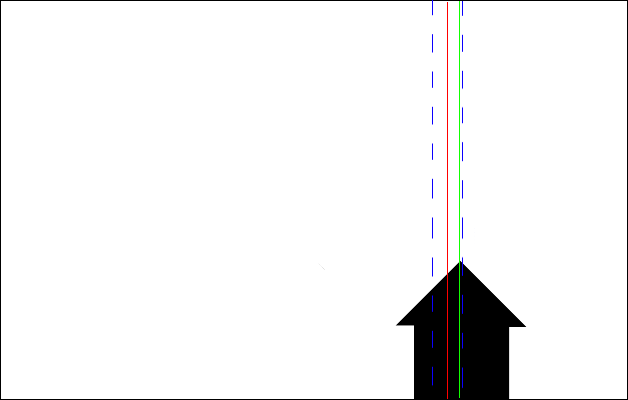
\includegraphics[scale=0.3,angle=0]{afsnit/vores_implementation/billeder/udvidet_loesning/husworks.png}
	\end{center}
	\caption[]{Et hus som bliver skåret over, så midten ligger inde for
    snittets margin.}
	\label{hus}
\end{figure}

\subsubsection{Opdeling af region med et gitter}
Vi bruger ikke længere regionens begrænsende rektangel, til at beskrive
regionen, så har vi brug for en anden måde at repræsentere denne på. Vi
laver derfor en approksimation, af regionens form og udstrækning ved at
bruge et gitter.  Alt efter hvor finmasket dette gitter er, kan man
justere hvor præcis approksimationen af regionen skal være. Et eksempel
på et gitter, ses i figur \ref{grid}, hvor regionen beskrives ved de
punkter, hvor to linjer krydser, og befinder sig inden for regionen.

I praksis bruges det segmenterede billede fra floodfill-metoden, til at
konstruere regionens approksimation. Vi kontrollerer hver pixel, som er
en del af gitteret, i det begrænsende rektangel for en given region, om
denne har samme farve, som regionen er blevet tildelt. Vi finder da et
undersæt af punkter til at beskrive regionen.

\begin{figure}[h]
    \centering
    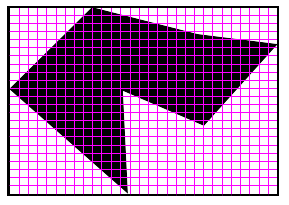
\includegraphics[scale=0.76,angle=0]{afsnit/vores_implementation/billeder/udvidet_loesning/udvidetloesninglayer.png}
    \caption[]{Et gitter over en regions begrænsende rektangel.}
    \label{grid}
\end{figure}

\subsubsection{Bedømmelse med hensyn til massemidtpunkt}
Givet en region $R$ betegner vi antallet af punkter i regionen med
$|R|$. Vi antager, at vi betragter et vertikalt snit $G$ i et billede.
Det gælder for alle punkter $p \in R$, at de kan befinde sig ovenpå,
til højre eller til venstre for $G$. I denne sammenhæng lader vi $R_r$
og $R_l$ beskrive punkter, henholdsvis til højre og venstre for snittet
$G$.  Afstanden fra et punkt til kanten af et billede kaldes $D_p$, hvor
kanten er origo i billedet.

Med disse informationer, kan vi afgøre, om snittet deler regionen i to
lige store dele, samt om store dele af regionen, befinder sig langt væk
fra snittet. Vi vil gerne kigge på en regions massemidtpunkt, og se om
dette ligger inden for margin.

\begin{definition}
    En regions massemidtpunkt er givet ved
    \begin{eqnarray}
        m(R) & = & \frac{\sum_{p \in R}{D_p}}{|R|} \label{masssemidpunkt}
        \label{MPunkt}
    \end{eqnarray}
    hvor $m(R)$ giver os en værdi for, hvilken lige linje, der deler
    regionen op i to dele, som er mest ens.
    \label{def_massemidtpunkt}
\end{definition}

\begin{figure}[h]
    \begin{center}
        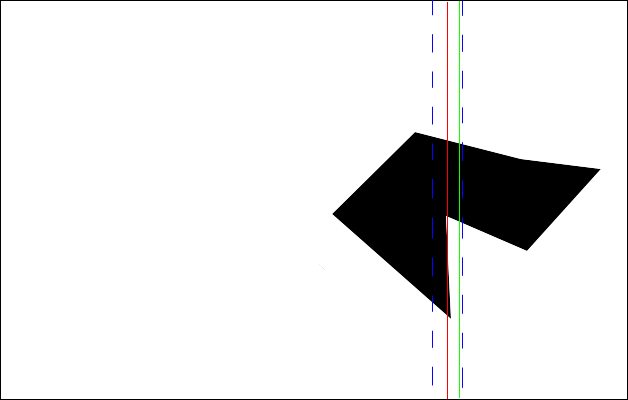
\includegraphics[scale=0.5,angle=0]{afsnit/vores_implementation/billeder/udvidet_loesning/cOMCutMargin.png}
    \end{center}
    \caption[]{Region, hvor massemidtpunkt, snit og margin er tegnet
    ind. Det ses, at massemidtpunktet, tegnet med en grøn linje, ligger
    inde for margin.}
    \label{cOMCutMargin}
\end{figure}

Hvis $m(R)$ ligger inden for margin, som tilfældet i figur
\ref{cOMCutMargin}, siger vil vi gerna have at regionen klassificeres
som positiv. Det er imidlertid ikke nok, kun at bedømme regionerne efter
massemidtpunkt, da man kan konstruere regioner, som vi ikke vil godtage,
men som har massemidtpunkt inden for margin. Et eksempel på en sådan
region er vist i figur \ref{dontwork}, hvor selve fordelingen af
regionens masse er skæv.

\begin{figure}[h]
    \begin{center}
        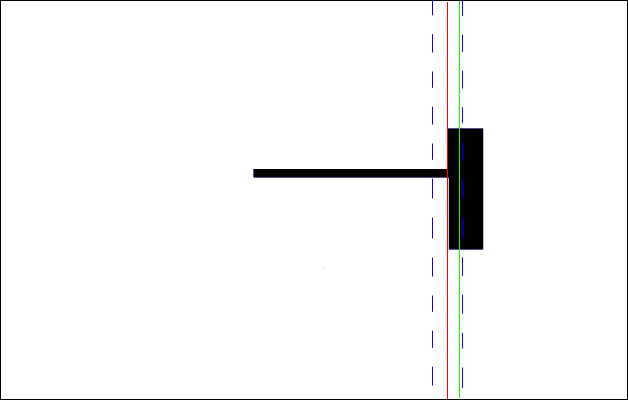
\includegraphics[scale=0.5,angle=0]{afsnit/vores_implementation/billeder/udvidet_loesning/dontWork.png}
    \end{center}
    \caption[]{Region, som har massemidtpunkt inden for margin, men som
    ikke kvalificerer sig til at ligge i snittet pga. arealets
    fordeling.}
    \label{dontwork}
\end{figure}

Vi forsøger at løse dette problem, ved at kontrollere regionens
fordeling over snittet.

\begin{definition}
    En regions fordeling over snittet findes ved
    \begin{eqnarray}
        f(R) & = & \frac{|R_{l}| - |R_{r}|}{|R|}
        \label{Fordeling}
    \end{eqnarray}
    \label{def_fordeling_ligning}
\end{definition}

\begin{definition}
    En region er jævnt fordelt over snittet, hvis forholdet mellem
    punkterne, på den højre og venstre side, er lavere en $75\%$.
    \label{def_fordeling_procent}
\end{definition}

I udregning \eqref{Fordeling} sammenlignes antal punkter, på begge sider af
snittet, og giver en procentsats for, hvor stor forskel der er mellem
siderne. Vi har at $f(R) \in [-1,1]$.  Hvis $f(R)$ er positiv, er der
$f(R)$ procent flere punkter på venstre side og vice versa. Her vises
netop hvorfor denne fremgangsmåde adskiller sig markant fra den naive.
Den naive fremgangsmåde søger nemlig at udvælge de regioner $R$, hvor
størstedelen af punkter ligger på den ene side af snittet, dvs. $|f(R)|
\geq 75\%$. Den udvidede løsning gør nøjagtig det modsatte og finder
regioner som er jævnt fordelt over snittet.

Vi bruger nu ovenstående til at definere, hvornår en region ligger i
snittet.

\begin{definition}
    Hvis en region er jævnt fordelt over snittet og har et
    massemidtpunkt inden for margin, så ligger denne region i snittet.
    \label{def_expanded}
\end{definition}

% Fjernet, da dette vil være første gang vi viser et egentligt resultat.
% Man ved ikke hvad man ser. Sådanne billeder bør vente til afprøvning.
%
%Få
%at give et eksempel på hvornår vores naive algoritme virker, se figur \ref{centerOfMass}
%\begin{figure}[h]
%	\begin{center}
%		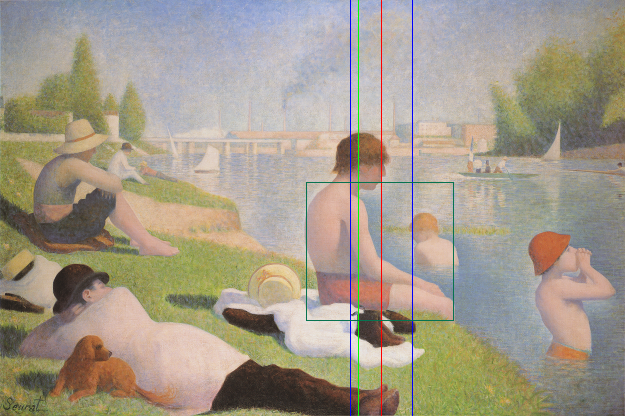
\includegraphics[scale=0.35,angle=0]{afsnit/vores_implementation/billeder/udvidet_loesning/centerOfMass.png}
%	\end{center}
%	\caption[]{Eksempel på hvordan den udvidet algoritme virker på et billedet hvor den naive algoritme ikke vil have fundet det}
%	\label{centerOfMass}
%\end{figure}

}

% vim: set tw=72 spell spelllang=da:


\subsection{Topografisk kort til omkostninger}
{
Et topografisk kort er et udtryk hentet fra geografi som er en
fremstilling af tærrenforskelle i et landskab. Traditionelle
topografiske kort bruger forskellige farver til at præsentere de
relative højder over havet. Denne metode kan bruges i andre sammenhænge,
f.eks. som vi vil gøre, ved at udskifte højde med en omkostning.
Eksempler på topografiske kort til klassificering af regioner i billeder
kan ses i figur \ref{topography_plus} og \ref{topography_times}.

Vi vil nu beskrive en metode hvorved regioner bliver tildelt en
omkostning. Denne omkostning beregnes ud fra regionens placering i
billedet på baggrund af et topografisk kort. Således vil regioner ikke
blive vurderet efter hvorvidt de ligger i det gyldne snit eller ej, men
efter \emph{hvor meget} de ligger i det gyldne snit.

\subsubsection*{Generering af topografisk kort}

Givet en afbildning af et maleri ved matricen $\mathbf{I}$ med dimensioner
$N \times{} M$, kan man opstille et topografisk kort $\mathbf{T}$ med dimensioner
$N \times{} M$.

Det topografiske kort generes ud fra to vektorer $\mathbf{X}^t =
\left(x_1, x_2, \cdots, x_n\right)$ og $\mathbf{Y} = \left(y_1, y_2,
\cdots, y_m\right)$ med dimensioner på henholdsvis $N \times 1$ og $1
\times M$.

Vi betragter vektoren $\mathbf{X}$ som liniestykket givet ved $AB$ i
figur \ref{topograph_line}. Længden af liniestykket betegnes ved $|AB|$.
Det følger af definitionen på $\mathbf{X}$ at $|AB| = n$. På liniestykket $AB$
er det gyldne snit placeret ved $G$ hvilket betegner indeks $\lfloor
n\varPhi \rfloor$ i $\mathbf{X}$. Et margin er angivet ved punkterne $(G
- \delta) = m$ og $(G + \delta) = m'$, hvor $\delta$ er størrelsen på
margin. Ligeledes betegner $m$ og $m'$ indeks $\lfloor n \varPhi \pm
\delta \rfloor$ i $\mathbf{X}$.  Endvidere har vi at $|Ap| = \lfloor
\frac{1}{2}|AB| \rfloor \leq |pB|$ og $|m'q| = \lfloor \frac{1}{2}|qB|
\rfloor \leq |qB|$. I figur \ref{topograph_line} er kun liniestykket
$pB$ segmenteret, men $Ap$ segmenteres symmetrisk.

Vi placerer nu et nyt punkt $x$ på $pB$. I det et-dimensionelle plan kan
længden $|Gx|$ bruges som mål for hvor tæt $x$ er på det gyldne snit.
Punktet $x$ har dog ingen udstrækning, hvorfor vi ikke blot kan bruge
længden i praksis. Vi betragter nu en region $R \in \mathbb{Z}^{+}$.
Regionen $R$ er en liniestykke i det et-dimensionelle plan. Vi kan da
udregne placeringen af $R$ i forhold til punktet $G$ ved at summere alle
afstandene fra punkterne $x$ i $R$ til $G$.  Dette medfører at lange
liniestykker bliver tildelt højere værdi end små. Vi udregner således
$\frac{\sum_{x \in R}{|Gx|}}{|R|} = |G(\frac{|R|}{2})|$, hvor $|R|$ er
længden, dvs. antallet af punkter i $R$. Dette svarer til at beregne
afstanden fra regionen midtpunkt til $G$. Dette er ikke ønskværdigt, da
vi kan have to regioner med forskellig længde, men med samme midtpunkt.
Hvis vi lader $R_{max}$ betegne den større region og $R_{min}$ være den
mindre, hvor $ \frac{|R_{max}|}{2} = \frac{|R_{min}|}{2}$, da må
$R_{max}$ nødvendigvis have et ekstrema tættere på $G$ end $R_{min}$.
Det er derfor ikke retfærdigt at give begge regioner den samme værdi.

Vi ønsker at belønne punkter der ligger i eller tæt ved det gyldne snit,
men give stor omkostning til punkter som ikke ligger i det gyldne snit.
Til dette bruges vektoren $\mathbf{X}$ angiver omkostningen for hvert
punkt på liniestykket $AB$. Da vi ønsker at belønne punkter i det gyldne
snit, tildels der ingen omkostning. Vi sætter derfor $\mathbf{X}_{|AG|}$
til $0$. Vi ønsker heller ikke at straffe regioner som ligger inden for
margin alt for meget. Vi sætter derfor $\mathbf{X}_{|Am|} =
\mathbf{X}_{|Am'|} = 1$, hvilket angiver omkostningen for at ligge på
margin. Værdierne mellem det gyldne snit og margin interpoleres således
at vi har en lineær overgang. Passende værdier vælges til
$\mathbf{X}_{|Ap|}$, $\mathbf{X}_{|Aq|}$ og $\mathbf{X}_{0} =
\mathbf{X}_{|AB|}$, hvor der ligeledes interpoleres mellem punkterne.
Liniestykket bliver således delt ind i nogle sektorer, som har en vis
omkostning alt efter hvor tæt man ligger på snittet. Derved kan vi undgå
ovenstående eksempel, hvor to regioner gives samme omkostning på trods
af at de har forskellig størrelse.

\begin{figure}[!h]
    \centering
    \begin{picture}(240,30)
        \put(0, 10){$A$}
        \put(3, -5){\line(0, 1){10}}

        \put(116, 10){$p$}
        \put(118, -5){\line(0, 1){10}}

        \put(131, 10){$m$}
        \put(134, -4){\line(0, 1){8}}

        \put(144, 10){$G$}
        \put(147, -4){\line(0, 1){8}}

        \put(157, 10){$m'$}
        \put(160, -4){\line(0, 1){8}}

        \put(195, 10){$q$}
        \put(198, -4){\line(0, 1){8}}

        \put(233, 10){$B$}
        \put(236, -5){\line(0, 1){10}}

        \put(182, 10){$x$}
        \put(185, 0){\circle*{3}}

        \put(3, 0){\line(1, 0){233}}
    \end{picture}
    \caption[]{Liniestykke}
    \label{topograph_line}
\end{figure}

\paragraph{Omkostningsfunktionen}
Vi vil nu overføre det ovenstående til to dimensioner. Det er trivielt
at opdele vektoren $\mathbf{Y}$ på samme måde som $\mathbf{X}$. Vi
ønsker at beregne en omkostning ud fra værdierne i vektorerne ved en
given koordinat. Vi definerer en funktion $t :
\mathbb{Z}^{+} \times \mathbb{Z}^{+} \rightarrow \mathbb{R}_{0}$ ved
\begin{equation}
    t(x, y) = \mathbf{X}_x + \mathbf{Y}_y
    \label{topo_plus}
\end{equation}
Det topografiske kort, som angivet ved funktionen \ref{topo_plus}, kan
ses i figur \ref{topography_plus}. Omkostninger er illustreret ved
mængden af hvid farve. Kortet viser at der ikke er nogen omkostning i
punktet $(G, G)$. Endvidere ses det at omkostningen er høj for punkter
ved hjørnerne og ved kanterne generelt. Dog kan man ret tydeligt se
grænserne mellem regionerne, da der interpoleres lineært.

Vi kan lave en mere flydende overgang mellem regionerne ved at definere
en ny funktion $u : \mathbb{Z}^{+} \times \mathbb{Z}^{+} \rightarrow
\mathbb{R}_{0}$ ved
\begin{equation}
    u(x, y) = \mathbf{X}_x\mathbf{Y}_y
    \label{topo_multiply}
\end{equation}
hvor vi multiplicerer omkostningerne i stedet for at addere dem. Det
resulterende topografiske kort ses i figur \ref{topography_times}. Da vi
nu bruger multiplikation vil vi gange med $0$ i det gyldne snit, hvorfor
dette er meget mere fremstående. Det skal dog nævnes at det ikke er helt
hensigtsmæssigt at omkostningen er meget lav ude ved ekstremerne.
Funktionen $u$ mangler altså den gode egenskab fra $t$ hvor ekstremerne
har store omkostninger.  Vi ser dog en eksponentiel stigning i
omkostningerne når vi bevæger os længere væk fra det gyldne snit.
Optimalt ville man have den samme omkostning ved ekstremerne som i $t$,
men med den eksponentielle stigning som i $u$.

Vi kan nu beregne omkostningen for en interessant region. Givet en
mængde $R \in \{\mathbb{Z}^{+}\times\mathbb{Z}^{+}\}$, som angiver
punkterne i en region, kan man finde omkostningen $C$ ved
\begin{equation}
    C(R) = \sum_{(x, y) \in R}{\frac{\tau(x, y)}{|R|}}
\end{equation}
hvor $\tau$ er en funktion fra $\mathbb{Z}^{+}\times\mathbb{Z}^{+}$ ind
i $\mathbb{R}_0$ som beregner omkostningen for et punkt fra et
topografisk kort. Vi har foreslået funktionerne $t$ og $u$. Jo lavere
omkostning en region har, jo bedre er den placeret i forhold til det
gyldne snit. I praksis er det oplagt at approksimere regionens
størrelse ved at bruge et gitter, ligesom i det foregående afsnit.


\begin{figure}[h]
    \setlength\fboxsep{0pt}
    \setlength\fboxrule{0.5pt}
    \begin{center}
        \fbox{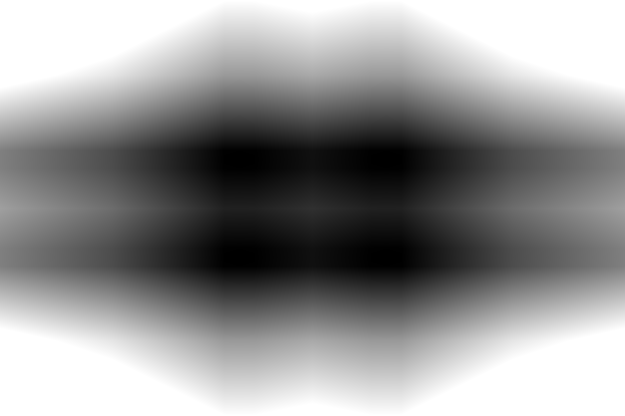
\includegraphics[width=0.8\textwidth]{afsnit/vores_implementation/billeder/udvidet_loesning/topographic_plus.png}}
    \end{center}
    \caption[]{Topografisk kort angivet ved funktionen $t(x, y) =
    \mathbf{X}_x + \mathbf{Y}_y$. Mængden af hvid farve reflekterer
    omkostningen. Helt hvid er dyrest, mens sort er billigst.}
    \label{topography_plus}
\end{figure}

\begin{figure}[h]
    \setlength\fboxsep{0pt}
    \setlength\fboxrule{0.5pt}
    \begin{center}
        \fbox{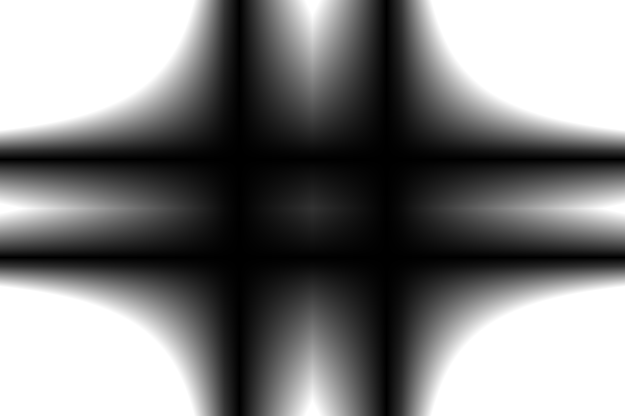
\includegraphics[width=0.8\textwidth]{afsnit/vores_implementation/billeder/udvidet_loesning/topographic_times.png}}
    \end{center}
    \caption[]{Topografisk kort angivet ved funktionen $u(x, y) =
    \mathbf{X}_x\mathbf{Y}_y$. Vi har igen, at hvid farve reflekterer
    omkostningen. Bemærk hvordan det gyldne snit er fremhævet.}
    \label{topography_times}
\end{figure}

\subsubsection*{Fastsættelse af omkostninger}
Det er let at se, at udformningen af det topografiske kort ikke blot
afhænger af funktionen $\tau$, men mere af de værdier man tildeler
omkostningsvektorerne. Værdierne, som er tildelt i det ovenstående, er
valgt arbitrært efter det bedste grafiske resultat. Vi har tidligere
nævnt, at værdierne interpoleres lineært. Hvis man adderer værdierne er
denne metode ikke helt hensigtsmæssig. Det er dog oplagt at gøre brug af
normalfordelingen til at fastsætte omkostninger. Dette skal dog ses med
omvendt fortegn, hvilket betyder, at vi nu tildeler regioner points. Man
kan altså basere antallet af points for et punkt i det et-dimensionelle
plan, ved at bruge en normalfordeling $N(\mu, \sigma)$ med middelværdi
$n\varPhi$ og en passende varians til margin. Umiddelbart ville man
sætte standardafvigelsen til $\delta$, vores margin, hvilket giver os en
varians på $\sigma^{2} = \delta^{2}$. Dette giver os en meget spids
normalfordeling, hvor punkter bliver tildelt mange points for at ligge
inden for margin, men hurtigt aftager når man bevæger sig længere væk.

%\subsubsection*{Fordele og ulemper}
%Brug af omkostninger ved topografiske kort har den umiddelbare fordel at
%kunne tildele regioner en værdi og derved være mere nuanceret i
%bedømmelsen af regioner. Metoden afhænger dog af fornuftige værdier i
%omkostningsvektorerne.

}

% vim: set tw=72 spell spelllang=da:


\subsection{Implementering af udvidelser}
Vi har valgt at implementere den først nævnte udvidelse til bedømmelse
af interessante regioner. Denne er valgt, da den er en simpel
modifikation af den eksisterende metode, hvilket gør, at vi også kan
afprøve metoden på vores korpus. Strukturen i metoden med topografiske
kort er meget langt væk fra den eksisterende metode, hvorfor vi har
vurderet, at denne ikke skulle implementeres. Topografiske kort indfører
også et mål på regionerne, hvilket vi ikke benytter os af i den
eksisterende metode.

}

% vim: set tw=72 spell spelllang=da:

